\documentclass[letterpaper,10pt]{article}

\usepackage[english]{babel}
\usepackage[utf8]{inputenc}
\usepackage{amsmath}
\usepackage{graphicx}
\usepackage[colorinlistoftodos]{todonotes}
\usepackage[top=0.5in, bottom=0.5in, left=1in, right=1in]{geometry}
\usepackage[small]{titlesec}

\newcommand{\bes}{\begin{equation*}}
\newcommand{\ben}[1]{\begin{equation}\label{#1}}
\newcommand{\ees}{\end{equation*}}
\newcommand{\be}{\begin{equation}}
\newcommand{\ee}{\end{equation}}

\begin{document}

\begin{flushright}
{\Large Josh Bevan - Midterm Project - CS555}
\end{flushright}
\vskip -0.1in
\hrule
\vskip 0.3in

\section*{Introduction}
The Euler equations describe inviscid, compressible fluid flow. It is possible to write the model equation as a system of scalar conservation laws, where the conserved quantities are the primitive variables $u,v,p$ (components of the flow velocity and pressure respectively). Hyperbolic equations of this type can be solved using a finite volume (FV) scheme. One notable advantage of a FV scheme over a finite difference scheme is the ease of use of unstructured meshes, which permit greater geometric freedom for representing boundary geometry.

This project implements a 2D unstructured FV scheme. It's measured error and order of convergence is examined for an analytical test case with a series of refined regular meshes. The developed solver is then used to examine a more difficult test case involving the propagation of a Gaussian pressure pulse on a mesh with complicated boundary geometry.

\section*{Implementation Details}
In conservation form the Euler equations are:
\begin{figure}[!htb]

\includegraphics[width=1\textwidth]{1.PNG}
\end{figure}

For 2D we can express this as a system of equations:

\begin{figure}[!htb]

\includegraphics[width=1\textwidth]{2.PNG}
\end{figure}

We can use a rotation of coordinates on the computational cell (with the mapping transforming $A,B \rightarrow C,D$) to eliminate one of the rotated components ($\hat{y}$ direction and it's associated mapped matrix $D$) to obtain:

\begin{figure}[!htb]

\includegraphics[width=1\textwidth]{3.PNG}
\end{figure}

where the mapped matrix $C$ is:

\begin{figure}[!htb]

\includegraphics[width=1\textwidth]{4.PNG}
\end{figure}

We can then diagonalize this using the eigenvectors of C, so that:

\begin{figure}[!htb]

\includegraphics[width=1\textwidth]{5.PNG}
\end{figure}
\newpage
After careful consideration of the flux through our computational element's boundary, and then mapping back to the physical element, we find that the (diagonalized) system of equations has become:

\begin{figure}[!htb]

\includegraphics[width=1\textwidth]{6.PNG}
\end{figure}

If we observe the fact that $\Lambda - |\Lambda|$ has only one non-zero entry in the middle element, the system of equations simplifies to:
\begin{figure}[!htb]
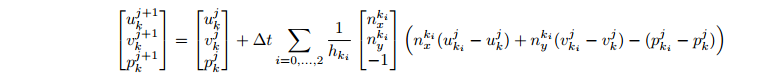
\includegraphics[width=1\textwidth]{7.PNG}
\end{figure}

Now we calculate the cell normals, the edge associated cell heights, and create a list of cell conserved quantity values and the cells that neighbor each cell edge. From this we compute the rate of change of the conserved quantities for all cells (for the current time step) and time step forward with a simple ``forward Euler'' time discretization scheme.

\section*{Results}

\subsection*{Analytical Test Case}
To first validate the solver and examine the order of convergence, an analytical test case is considered. On a square domain with reflective boundary conditions, the initial conditions:
\begin{figure}[!htb]

\includegraphics[width=1\textwidth]{8.PNG}
\end{figure}

permit analytical solutions of the form:
\begin{figure}[!htb]

\includegraphics[width=1\textwidth]{9.PNG}
\end{figure}

This test case was examined for the square/square2/square.neu meshes as well as intermediate meshes that were result of applying refine\_mesh.refine2dtri() to the first two meshes. This resulted in five meshes with element numbers increasing as: 226, 904, 4096, 16384, 65536.

For each of these meshes, the time step was chosen to be $\sim 0.25 \, h_{min}$. All runs were allowed to evolve for 3.2s, and the time step for each was chosen near to the given step size relation, but also to be able to evenly divide the time step of the coarsest mesh. This is necessary if one would like to directly compare the time varying errors or each run to each other to calculate a time varying order of convergence.

\subsection*{A Careful Consideration of Error Measures}
To determine the order of convergence, three measures of errors were considered. All errors were based on the l2 discrete norm. For reference, Figure 2 shows a plot of all three errors for an example mesh.

The most straightforward error measure used was the norm of the absolute error between the computed and exact solutions. For solutions where the conserved quantity is strictly positive this would be a sufficient error to use to determine convergence. However in this test case the relative pressure is free to be both positive and negative. Additionally, the reflective boundary conditions result in periodic destructive interference between the reflected pressure waves. The result is that at regular intervals the magnitude of the pressure everywhere in the domain is close to zero. The consequence of this is that the absolute error periodically dips to nearly zero, despite the fact that in actuality the computed quantities aren't any more accurate.

A relative error would then seem to be more appropriate, so that the error calculated is relative to the time varying magnitude of pressure. Another issue arrives using this second error measure. As previously stated the magnitude of the pressure periodically approaches zero; by numerical chance some of cell values can be even closer to zero than average resulting in locally high relative errors that are due mostly to their sensitivity in small absolute perturbations, that are large nevertheless in the relative sense. Referring to Figure 2 we can see that where the magnitude of the pressure drops to nearly zero the absolute error also becomes nearly zero, but this is due to the relative change in pressure. At these corresponding times, we can see spurious spikes in the ``unfiltered'' relative error, where small absolute perturbations in the computed solution are large relative to the small values of the analytical solution.

The final error measure seeks to mitigate these spurious oscillations by filtering the peaks in the relative error. For this purpose a 1-st order Butterworth filter was used, with a normalized low pass cutoff frequency of 0.03. Again referring to Figure 2 we can see the low pass filter eliminates the spurious peaks in the relative error, while preserving the low frequency, meaningful behavior of the time evolution of the norm of the error.

\subsection*{Application of Error Measures to Analytical Results}
We can now apply our three error measures to examine the time varying order of convergence of the method applied to the stated analytical test case. Figure 1 plots this time evolution, where the computed order of convergence is the result of a log-log polynomial fit for the five meshes at each time level. The first most evident feature is that despite the difference in approaches, all three error measures roughly agree in the bulk; nominally the order of convergence is $\sim 0.5$. As might be expected, the absolute error measure is the most pessimistic of the three. This should be evident when one considers that during times near when the pressure waves destructively cancel, the computed absolute error is quite low for all mesh sizes. If mesh size has a weaker effect on convergence, then one should expect a lower observed order of convergence.

By comparison, the unfiltered relative error more fairly represents convergence where the numerical error in the computed solution is close in magnitude to the actual value of the solution. Despite this more fair assessment the measure is sensitive to error outliers that are not a consequence of the actual solver performance. The order of convergence computed from the filtered relative norms is arguably the most fair for all time levels. At times where the magnitude of the solution is large, the order of convergence based on the filtered relative error reproduces the unfiltered relative error order of convergence. At times where the unfiltered relative error succumbs to spurious peaks, the order of convergence based on the filtered relative error remains a good approximation for the effective order of convergence.

\begin{figure}[!htb]
\centering
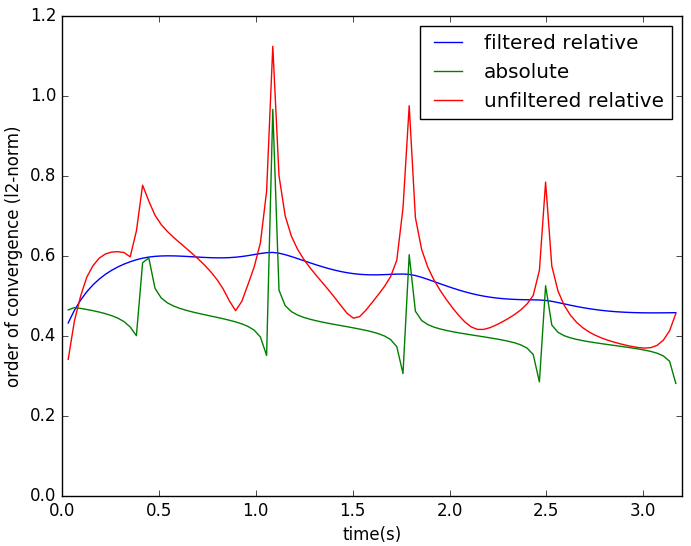
\includegraphics[width=0.75\textwidth]{timeconv.PNG}
\caption{\label{fig:unrolled}Time varying order of convergence for analytical test case, based on 5 mesh refinement levels.}
\end{figure}

\begin{figure}[!htb]
\centering
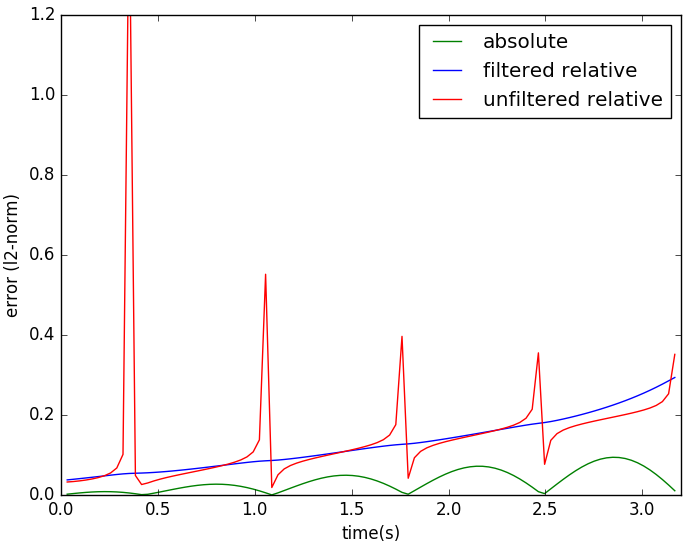
\includegraphics[width=0.75\textwidth]{error3.PNG}
\caption{\label{fig:unrolled}Example error plot (for square3.neu mesh), showing time varying absolute and relative errors, notably spurious relative error behavior where the analytical solution is nearly zero.}
\end{figure}

\newpage

\subsection*{Stability for Analytical Test Case}
The stability condition expected numerically for the problem is $\Delta t \leq C min(h^{k_i}), \, C=0.5$. Empirically, it was observed that the maximum coefficient allowable was around 0.4 to 0.42. This can partly be explained due to the finite floating point precision and roundoff inherent computationally; the ideal limit is based on a scheme using exact values and no roundoff.

The combination of limited precision and roundoff leads to small perturbations in computed values. In some cases the perturbations may be dissipative, but in others they may lead to small amplifications. The propagation/accumulation of these small amplifications may lead to premature breakdown of the solver for what would seem to be time step sizes within the CFL limits.

\subsection*{Coastal Mesh Pressure Pulse Test Case}
While the previous test case has the advantage that an analytical solution exists for comparison with the computed solution, the mesh on the square domain doesn't fully exercise the potential capabilities (or expose issues) of the solver. The other test case involves a Gaussian pressure pulse $p(x,y) = exp(-(x-200)^2+(y+400)^2/10000)$ on a mesh generated from the coastline or Ireland.

For this test case the time step was again set to be $\Delta t=0.25 \, h_{min}$. Figures 3 and 4 show the initial pulse and the pulse after 450 seconds. Qualitatively the solution seems to make sense. The pulse traveled radially outward until it contact domain boundaries. The boundary conditions are such that the pulse reflected, and these reflections can be seen in Figure 4. along the southwest boundary part of the arc of the pulse can be seen traveling back towards the pulse center after reflecting.

An additional physical feature of interest is the concentration of the pressure wave in the narrow passage on the east side of the domain. The funnel shape of the passage concentrates the pressure wave to a locally high pressure, which would seem to make sense. This concentration bears some real world significance if one thinks of the pressure wave in this simulation as an analogue to a water wave, where wave height is proportional to pressure. The funnel area is actually the Severn estuary, the pressure concentration is an area called the Severn bore. The Severn bore is notable for the strong tidal action that occurs where tidal action is concentrated by the geography. By this analogy the results seem to make sense.

One final consideration is the appropriateness of the size of the domain. With the given mesh depending on what time and point is of interest the domain may be too small. Unwanted boundary reflections may eventually confound the desired results since the northwest and southwest boundaries aren't actually coastline, but computational boundaries.

\begin{figure}[!htb]
\centering
\includegraphics[width=0.8\textwidth]{captureT0.PNG}
\caption{\label{fig:unrolled}Coastline initial conditions, gaussian pulse at t=0.}
\end{figure}

\begin{figure}[!htb]
\centering
\includegraphics[width=0.8\textwidth]{captureTAB.PNG}
\caption{\label{fig:unrolled}Pulse at t=450s, showing reflections at domain boundary. Left n=27808, right n=111232 }
\end{figure}
\newpage

Figure 4 compares the solution on the original mesh and a refined mesh. The two are in general agreement, implying the coarser mesh is likely sufficiently converged to trust. There are small noticeable differences between the two when one examines the width of the expanding wave from the pulse. The solution on the finer mesh appears to be more coherent and to have spread slightly less, but isn't notably different.

\subsection*{Conclusion}
A finite volume solver was constructed for the solution of Euler's equations. The solver was examined for an analytical test case and found to have an order of convergence of nominally 0.5, and a CFL limit of around 0.41. The solver was also applied to a more Gaussian pulse on a more challenging domain and found to perform at least qualitatively correctly. Wave reflections and geometry induced concentrating effects were observed which match physical intuition.

\end{document}

%\begin{figure}[!htb]
%\centering
%\includegraphics[width=0.6\textwidth]{Unrolled.PNG}
%\caption{\label{fig:unrolled}"Unrolled" ring, coincident nodes at either end.}
%\end{figure}